\documentclass[8pt]{article}
\usepackage[utf8]{inputenc}
\usepackage{color, hyperref, amsmath, graphicx} %, Rd}
\usepackage{framed}
\usepackage{alltt}

\setlength{\oddsidemargin}{0in}
\setlength{\topmargin}{0in}
\setlength{\textwidth}{6.5in} \setlength{\textheight}{8.5in}

%% maxwidth is the original width if it is less than linewidth
%% otherwise use linewidth (to make sure the graphics do not exceed the margin)
\makeatletter
\def\maxwidth{ %
	\ifdim\Gin@nat@width>\linewidth
	\linewidth
	\else
	\Gin@nat@width
	\fi
}
\makeatother

\definecolor{fgcolor}{rgb}{0.345, 0.345, 0.345}
\newcommand{\hlnum}[1]{\textcolor[rgb]{0.686,0.059,0.569}{#1}}%
\newcommand{\hlstr}[1]{\textcolor[rgb]{0.192,0.494,0.8}{#1}}%
\newcommand{\hlcom}[1]{\textcolor[rgb]{0.678,0.584,0.686}{\textit{#1}}}%
\newcommand{\hlopt}[1]{\textcolor[rgb]{0,0,0}{#1}}%
\newcommand{\hlstd}[1]{\textcolor[rgb]{0.345,0.345,0.345}{#1}}%
\newcommand{\hlkwa}[1]{\textcolor[rgb]{0.161,0.373,0.58}{\textbf{#1}}}%
\newcommand{\hlkwb}[1]{\textcolor[rgb]{0.69,0.353,0.396}{#1}}%
\newcommand{\hlkwc}[1]{\textcolor[rgb]{0.333,0.667,0.333}{#1}}%
\newcommand{\hlkwd}[1]{\textcolor[rgb]{0.737,0.353,0.396}{\textbf{#1}}}%

\usepackage{framed}
\makeatletter
\newenvironment{kframe}{%
	\def\at@end@of@kframe{}%
	\ifinner\ifhmode%
	\def\at@end@of@kframe{\end{minipage}}%
\begin{minipage}{\columnwidth}%
	\fi\fi%
	\def\FrameCommand##1{\hskip\@totalleftmargin \hskip-\fboxsep
		\colorbox{shadecolor}{##1}\hskip-\fboxsep
		% There is no \\@totalrightmargin, so:
		\hskip-\linewidth \hskip-\@totalleftmargin \hskip\columnwidth}%
	\MakeFramed {\advance\hsize-\width
		\@totalleftmargin\z@ \linewidth\hsize
		\@setminipage}}%
{\par\unskip\endMakeFramed%
	\at@end@of@kframe}
\makeatother

\definecolor{shadecolor}{rgb}{.97, .97, .97}
\definecolor{messagecolor}{rgb}{0, 0, 0}
\definecolor{warningcolor}{rgb}{1, 0, 1}
\definecolor{errorcolor}{rgb}{1, 0, 0}
\newenvironment{knitrout}{}{} % an empty environment to be redefined in TeX

% set up headers and footers
\usepackage{fancyhdr}
\pagestyle{fancy}
\lhead{PH 290: Project 2}
\chead{}
\rhead{Jin Rou New}
\lfoot{}
\cfoot{}
\rfoot{\thepage}

%% for inline R code: if the inline code is not correctly parsed, you will see a message
\newcommand{\rinline}[1]{SOMETHING WRONG WITH knitr}

\usepackage{titling}
\setlength{\droptitle}{-10em} % Remove spacing before title

\usepackage{titlesec}
\titlespacing{\section}{0pt}{\parskip}{-\parskip}
%\titlespacing{\subsection}{0pt}{\parskip}{-\parskip}
%\titlespacing{\subsubsection}{0pt}{\parskip}{-\parskip}

\title{PH290: Kaggle Predicting Parkinson's Disease Progression\\with Smartphone Data}
\author{Jin Rou New\\
	SID: 25944841
%	\\ University of California, Berkeley
	}
\date{\vspace{-5ex}} % Remove date to save space
%\date{\today}

\setlength\parindent{0pt}
\setlength{\parskip}{\baselineskip} % to get space between paragraphs
\usepackage{setspace} % to allow for double line spacing
\begin{document}
\maketitle
%\renewcommand{\abstractname}{}
%==================================================
%Data analysis: (a) summarize the winning methods; (b) propose your own
%solution and do a comparison; (c) carry out an analysis to address your
%own question.
%
%The report is no more than 3 pages, including tables and figures (and
%references, everything).
%{ At the beginning of the report, prepare a summary of your findings (what
%kind of useful knowledge you have obtained via your analysis).
%{ Make sure to include a description on how you process the data.
%==================================================
\section{Summary}
\label{sec:summary}
A number of classifiers, including LDA, QDA, SVM and RF were applied to hourly accelerometer data passively collected from 16 smartphone users, 9 of which have Parkinson's Disease (PD). The first three classifiers performed poorly, predicting the test/left-out user to have PD at every try. However, the RF had superior performance with 100\% prediction accuracy determined by leave-one-out cross validation. The RF hence shows promising results for predicting if a user has PD based on his/her accelerometer data.
%==================================================
\section{Introduction}
\label{sec:introduction}
The key aim of the Kaggle competition is to use the data collected from 16 smartphone users to distinguish Parkinson's Disease (PD) patients from healthy controls. Of the 16 users, 9 are PD patients at varying stages of the disease. The smarthphone data includes audio, accelorometry, compass, ambient light, proximity, battery level and GPS data.
%==================================================
\section{Data processing and feature engineering} 
\label{sec:data-processing}
The data is organized into about 7000 compressed folders each containing a set of csv and log files. I wrote a bash shell script to programmatically uncompress and concatenate csv files of each type of smartphone data for each user and discarded the log files. Ultimately, only accelerometer and GPS data were used in my analysis.

For both accelerometer and GPS data, I aggregated them by second (as multiple samples were usually available in one second) by taking the average for every variable. Next, for the accelerometer data, I aggregated them by hour and discarded hourly windows with less than 5 seconds of data. Finally, as pointed out by Wang (2012), since the x, y and z axes were measured with respect to the phone's orientation, which is unclear based on the accelerometer alone, I took the root mean square of the 3 channels for all variables.

The resulting data set has 4615 observations and 8 features aside from the class (PD vs Control) for the 16 users: average hourly mean acceleration, acceleration standard deviation, acceleration absolute deviation, acceleration maximum deviation, power spectral density (PSD) for 1Hz, 3Hz, 6Hz and 10Hz bands combined across all x, y and z axes (using root mean square). The relationship between each pair of variables is visualized in Figure~\ref{fig:pairs}. We see some separation between PD patients and healthy controls.

\begin{figure}[htb]
	\begin{center} 
		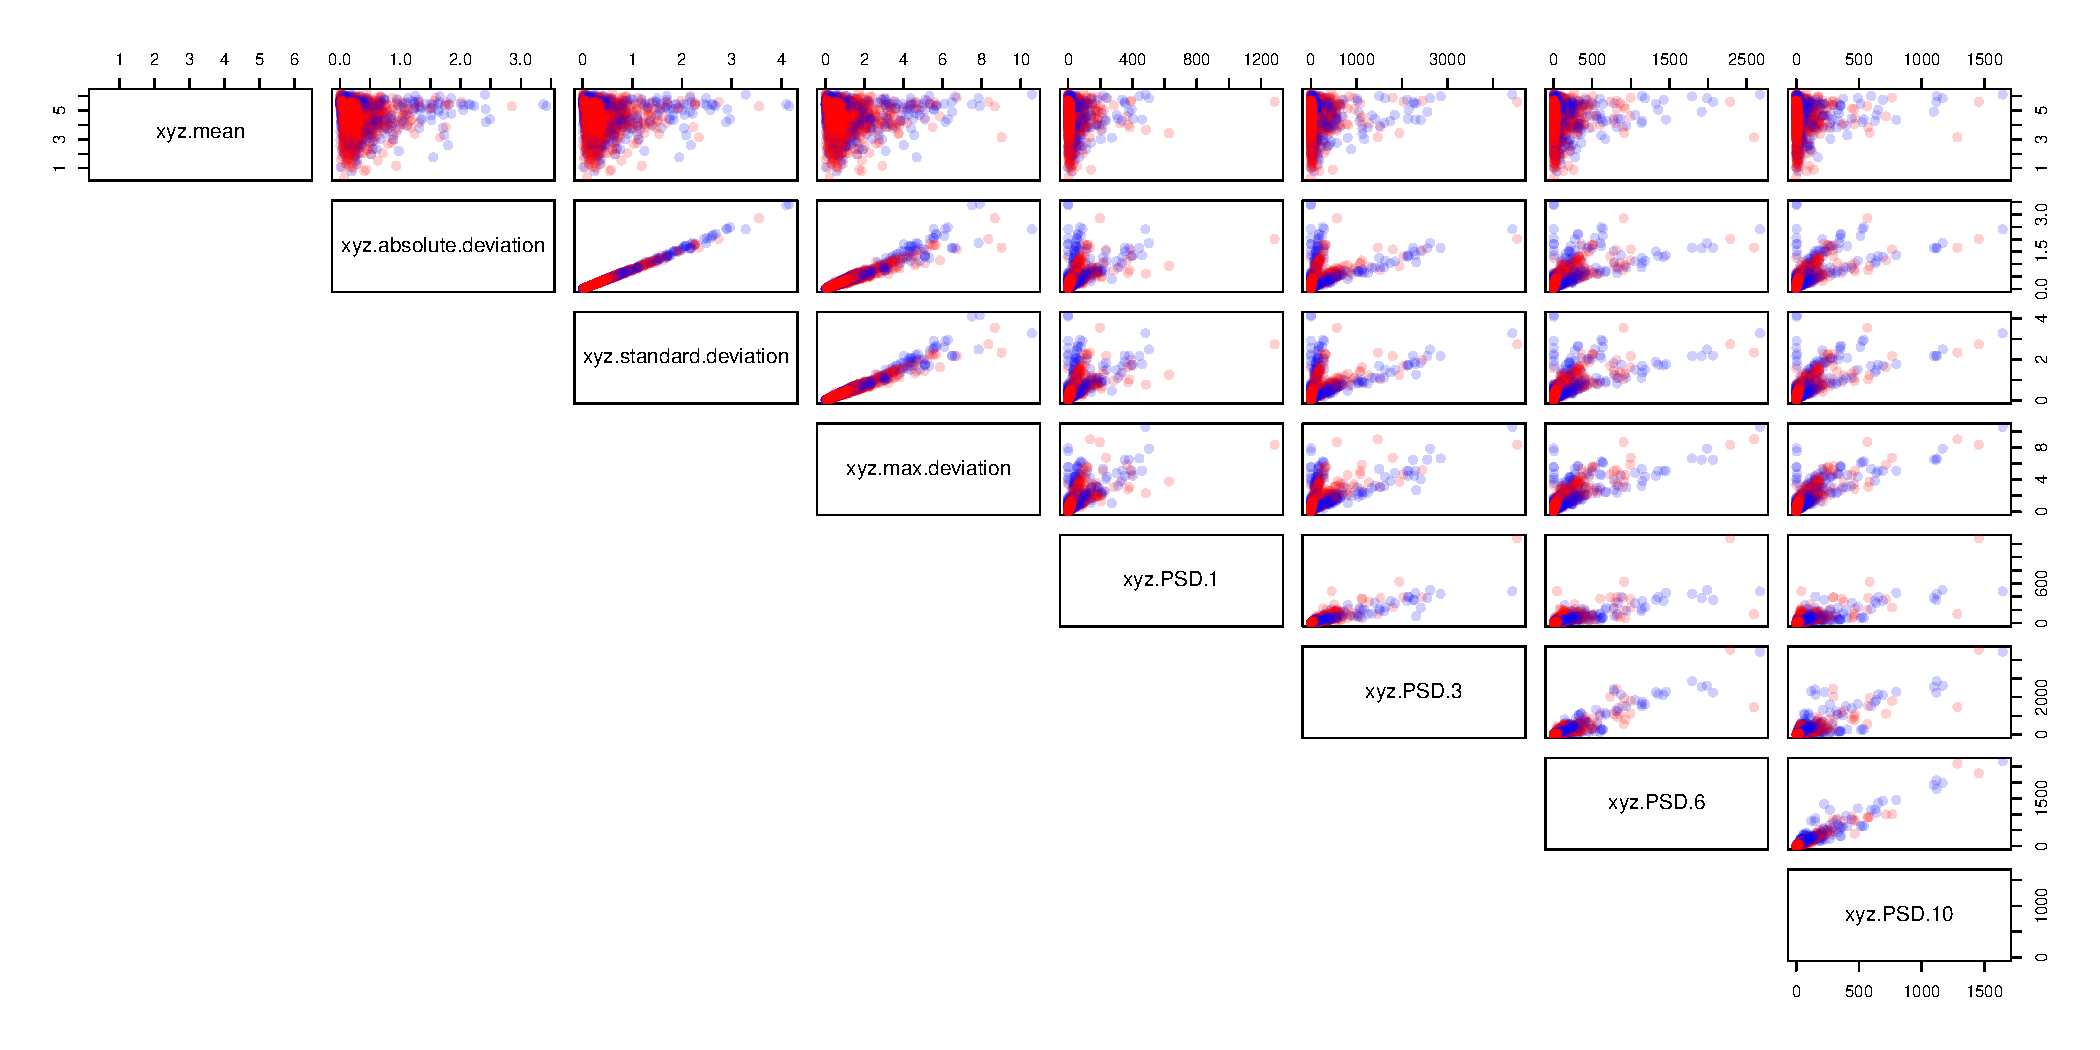
\includegraphics[width = 0.8\textwidth]{fig/pairs.pdf}
		\caption{{\bf Pairs plot of all 8 features for PD patients (in red) and healthy controls (in blue).}}
		\label{fig:pairs}
	\end{center}
\end{figure}
%==================================================
\section{Proposed method}
I applied a range of classification methods to the processed data set to determine the one that gave the best results, including Linear Discriminant Analysis, Quadratic Discriminant Analysis, Support Vector Machine and Random Forest (RF).

To assess the performance of each method, I used leave-one-out cross validation, as was also done by Brunato et al. (2012). Each classifier was trained with all data points except those of one user, and then used to predict the class of all data points of that left-out user. The proportion of of data points of that user that are predicted to have the ``PD'' class gives the probability that the user has PD. If that probability is more than half, that user is predicted to have PD. 

The first three classifiers performed poorly, predicting the test/left-out user to have PD in all 16 cases. However, the RF had superior performance with 100\% prediction accuracy, i.e. the test/left-out user was predicted correctly to be in either group in all 16 cases. Finally, I applied RF to the full data set and determined that the average hourly mean acceleration and PSD in the 6Hz band seem to be the most important variables.

%\begin{figure}[htb]
%	\begin{center} 
%		\includegraphics[width = 0.4\textwidth]{fig/rf-importance.pdf}
%		\caption{{\bf Variables ranked by variable relative importance for the model based on the Random Forest.}}
%		\label{fig:importance}
%	\end{center}
%\end{figure}

%All calculations were carried out in the R programming language, with additional functions from the \texttt{tidyr} and \texttt{dplyr} packages for data processing and from the \texttt{randomForest} and \texttt{gbm} packages for modelling. 
%==================================================
\section{Method benchmarking}
\label{sec:comparison}
Brunato et al. (2012) and Wang (2012) first applied k-means clustering to the compass and GPS data to identify windows in which the users were in motion. Accelerometer data from these windows were then discarded. A SVM was then applied to these data averaged in each window. With leave-one-out cross validation, they achieved 100\% prediction accuracy.

Wang averaged acceleration data over hourly windows and combined the x, y and z channels into one by taking their root mean square. He also used a SVM on the data with 5 features: the mean acceleration value and the PSD across 4 separate bands. The k-fold cross validation error for his classifiers were about 15\% and 9\% respectively.

Teo and Nachev (2012), on the other hand, opted for a simple hypothesis-driven univariate analysis of the data. They calculated the intersessional absolute deviation (ISAD) of the accelerometer mean for randomly selected 1-hour recording sessions and found that all users could be categorised into three groups based on their ISAD level: patients taking the medication levodopa, healthy controls and patients not on that medication.

With its 100\% prediction accuracy , my proposed method performed as well as Brunato et al. (2012)'s method, despite its comparative simplicity and its use of only the accelerometer data. A fair comparison of my method and the other two winning methods could not be made as different metrics were used, however, it does appear to be superior given the high prediction accuracy.
%==================================================
\section{Additional analyses}
\label{sec:addition}
I was interested in determining how much could be gleaned from GPS data of smartphone users. After reducing the GPS data to per-second data, I plotted the data by data for all users. An example series is shown in Figure~\ref{fig:gps} for the user Crocus. It was possible to determine the user's home, daily movement patterns and travel patterns by simply examining these plots over time. More sophisticated analyses could possibly determine the time spent at each location, guess at the mode of transport (e.g. car vs bicyle vs public bus/subway) taken by the user by calculating the speed of travel and comparing the routes taken with bus/subway maps. I tried to determine if the user is a PD patient or a healthy control based on the GPS data (the hypothesis being that someone with PD is likely to move around less). While my guess that Crocus is a healthy control is right, given that Crocus travels long distances frequently, this could not be generalized as there were many confounding variables such as age and occupation. Moreover, these raise important ethical questions and privacy concerns for the use and analysis of smartphone data as too much information aside from the study aims is revealed through the GPS data.

\begin{figure}[htbp]
	\begin{center}
		\includegraphics[width = 1\textwidth]{fig/gps_CROCUS1.pdf}
		\caption{{\bf Plot of GPS coordinates for user Crocus over three days. The blue and red spots show the starting and ending points respectively of each day.}}
		\label{fig:gps}
	\end{center}
\end{figure}
%==================================================
\section{Discussion} 
\label{sec:discussion}
While initial results indeed show a lot of potential, more training and testing of my proposed solution on data from a larger study group of smartphone users would be necessary to assess if the results can indeed be generalized to a larger population.
%==================================================
\section{References}
{\tiny
1. Brunato, M., Battiti, R., Pruitt, D. and Sartori, E. (2012). Supervised and unsupervised machine learning for the detection, monitoring and management of Parkinson's disease from passive mobile phone data. \\
2. Teo, J.T.H. and Nachev, P. (2012). Remote monitoring of Levodopa response in Parkinson's disease.\\
3. Wang, M. (2012). Identifying Parkinson’s Disease from Passively Collected Data.\\
}
\end{document}
